\documentclass[nobib]{tufte-handout}

%\\geometry{showframe}% for debugging purposes -- displays the margins

\newcommand{\bra}[1]{\left(#1\right)}
\usepackage{amssymb}
\usepackage{hyperref}
\usepackage{pgfplots}
\usepackage[activate={true,nocompatibility},final,tracking=true,kerning=true,spacing=true,factor=1100,stretch=10,shrink=10]{microtype}
\usepackage{color}
\usepackage{steinmetz}
\usepackage{placeins}
% Fixes captions and images being cut off
\usepackage{marginfix}
\usepackage{array}
\usepackage{tikz}
\usepackage{amsmath,amsthm}
\usetikzlibrary{shapes}
\usetikzlibrary{positioning}
\usetikzlibrary{circuits.logic.US}
\usepackage{listings}
\usepackage{forest}
\usepackage{caption}
\DeclareCaptionFont{white}{\color{white}}
\DeclareCaptionFormat{listing}{\colorbox{gray}{\parbox{\textwidth}{#1#2#3}}}
\captionsetup[lstlisting]{format=listing,labelfont=white,textfont=white}

% Set up the images/graphics package
\usepackage{graphicx}
\setkeys{Gin}{width=\linewidth,totalheight=\textheight,keepaspectratio}
\graphicspath{{.}}

\title{Notes for ECE 27000 - Introduction to Digital System Design}
\author{Zeke Ulrich}
\date{\today}  % if the \date{} command is left out, the current date will be used

% The following package makes prettier tables.  We're all about the bling!
\usepackage{booktabs}

% The units package provides nice, non-stacked fractions and better spacing
% for units.
\usepackage{units}

% The fancyvrb package lets us customize the formatting of verbatim
% environments.  We use a slightly smaller font.
\usepackage{fancyvrb}
\fvset{fontsize=\normalsize}

% Small sections of multiple columns
\usepackage{multicol}

% For finite state machines 
\usetikzlibrary{automata} % Import library for drawing automata
\usetikzlibrary{positioning} % ...positioning nodes
\usetikzlibrary{arrows} % ...customizing arrows
\tikzset{node distance=2.5cm, % Minimum distance between two nodes. Change if necessary.
    every state/.style={ % Sets the properties for each state
    semithick,
    fill=gray!10},
    initial text={}, % No label on start arrow
    double distance=2pt, % Adjust appearance of accept states
    every edge/.style={ % Sets the properties for each transition
    draw,
    ->,>=stealth', % Makes edges directed with bold arrowheads
    auto,
    semithick}}
\let\epsilon\varepsilon

% These commands are used to pretty-print LaTeX commands
\newcommand{\doccmd}[1]{\texttt{\textbackslash#1}}% command name -- adds backslash automatically
\newcommand{\docopt}[1]{\ensuremath{\langle}\textrm{\textit{#1}}\ensuremath{\rangle}}% optional command argument
\newcommand{\docarg}[1]{\textrm{\textit{#1}}}% (required) command argument
\newenvironment{docspec}{\begin{quote}\noindent}{\end{quote}}% command specification environment
\newcommand{\docenv}[1]{\textsf{#1}}% environment name
\newcommand{\docpkg}[1]{\texttt{#1}}% package name
\newcommand{\doccls}[1]{\texttt{#1}}% document class name
\newcommand{\docclsopt}[1]{\texttt{#1}}% document class option name

% Define a custom command for definitions and biconditional
\newcommand{\defn}[2]{\noindent\textbf{#1}:\ #2}
\let\biconditional\leftrightarrow

\begin{document}

\maketitle

\tableofcontents

\section{Course Description}
An introduction to digital system design, with an emphasis on
practical design techniques and circuit implementation.
\pagebreak

\section{Verilog}

SystemVerilog is a hardware description and verification language 
(HDVL) that extends Verilog by adding high-level programming constructs. 
It is widely used for modeling, simulating, and verifying digital 
systems.

The listing below is an example of a NAND gate expressed in SystemVerilog.

\begin{lstlisting}[caption={NAND}, label={lst:nand_gate}]
module nand_gate (
    input  logic a,
    input  logic b,
    output logic y
);
    assign y = ~(a & b);
endmodule
\end{lstlisting}

In SystemVerilog, numbers are written in format
\texttt{[size]'[base][number]}, for example:
\begin{itemize}
    \item 4'b1001 (binary, 9 in decimal, bit width 4 bits)
    \item 8'hf1 (hex, equals 421, bit width 8 bits)
    \item 3'o3 (octal, 3, bit width 3 bits)
    \item 32'b1001\_1101\_0101\_1111 (binary, 40255, bit width 32 bits)
\end{itemize}


\section{Number Systems}
In daily life, we primarily interact with the familiar
base-10 numbers. However, when interaction with digital
systems, we must also concern ourselves with base-2, base-8,
base-16, and other bases which are friendly to binary
states. Unless completely unambiguous, the base of a number
is written as a right subscript such as $144_{10}$ for base-10
or $1001_{2}$ for base-2.

For binary numbers, each digit represents a power of two.
To convert a binary number to decimal, you sum the products of
each binary digit with its corresponding power of two. For
example, the binary number 1001 is calculated as
\begin{align}
    2^3 \times 1 + 2^2 \times 0 + 2^1 \times 0 + 2^0 \times 1 & = 8 + 0 + 0 + 1 \\
                                                              & = 9_{10}
\end{align}

To convert from hexadecimal to decimal, each digit represents a
power of sixteen. For instance, the hexadecimal number f1 is
calculated as
\begin{align}
    15 \times 161+1 \times 160 & = 240+1    \\
                               & = 241_{10}
\end{align}
where f represents the decimal value 15.
When converting to another base, reverse the process by dividing
the decimal number by the target base, recording the remainder,
and repeating with the quotient until it reaches zero.
The remainders give you the digits of the number in the new
base, read in reverse order.

To convert a decimal number into binary, for example, you
repeatedly divide the number by 2 and record the remainders.
For the decimal number 9, dividing by 2 gives a quotient of 4
and a remainder of 1. Dividing 4 by 2 gives a quotient of 2
and a remainder of 0. Dividing 2 by 2 gives a quotient of 1
and a remainder of 0, and finally, dividing 1 by 2 gives a
quotient of 0 and a remainder of 1. Reading the remainders
from bottom to top, the binary representation of 9 is 1001.
\section{Boolean Algebra}
Computers operate in binary. To represent the state of a
computer we require a suitable mathematical framework,
provided by boolean algebra. In boolean algebra, variables 
can only take on two values: 0 and 1. 

\begin{table}[h]
    \centering
    \begin{tabular}{|l|l|}
        \hline
        \textbf{Rule}           & \textbf{Expression}                                                                            \\ \hline
        Commutativity           & $X + Y = Y + X$                                                                                \\
                                & $X \cdot Y = Y \cdot X$                                                                        \\ \hline
        Associativity           & $(X + Y) + Z = X + (Y + Z)$                                                                    \\
                                & $(X \cdot Y) \cdot Z = X \cdot (Y \cdot Z)$                                                    \\ \hline
        Distributivity          & $X \cdot Y + X \cdot Z = X \cdot (Y + Z)$                                                      \\
                                & $(X + Y) \cdot (X + Z) = X + Y \cdot Z$                                                        \\ \hline
        Covering                & $X + X \cdot Y = X$                                                                            \\
                                & $X \cdot (X + Y) = X$                                                                          \\ \hline
        Combining               & $X \cdot Y + X \cdot Y = X$                                                                    \\
                                & $(X + Y) \cdot (X + Y) = X$                                                                    \\ \hline
        Consensus               & $X \cdot Y + X \cdot Z + Y \cdot Z = X \cdot Y + X' \cdot Z$                                   \\
                                & $(X + Y) \cdot (X + Z) \cdot (Y + Z) = (X + Y) \cdot (X + Z)$                                  \\ \hline
        Generalized Idempotency & $X + X + \dots + X = X$                                                                        \\
                                & $X \cdot X \cdot \dots \cdot X = X$                                                            \\ \hline
        DeMorgan's Theorems     & $(X_1 \cdot X_2 \cdot \dots \cdot X_n)' = X_1' + X_2' + \dots + X_n'$                          \\
                                & $(X_1 + X_2 + \dots + X_n)' = X_1' \cdot X_2' \cdot \dots \cdot X_n'$                          \\ \hline
        Generalized DeMorgan's  & $F(X_1, X_2, \dots, X_n, +, \cdot) = F(X_1, X_2, \dots, X_n, \cdot, +)'$                       \\ \hline
        Shannon's Expansion     & $F(X_1, X_2, \dots, X_n) = X_1 \cdot F(1, X_2, \dots, X_n) + X_1' \cdot F(0, X_2, \dots, X_n)$ \\
                                & $F(X_1, X_2, \dots, X_n) = [X_1 + F(0, X_2, \dots, X_n)] \cdot [X_1' + F(1, X_2, \dots, X_n)]$ \\ \hline
    \end{tabular}
    \caption{Boolean Algebra}
    \label{tab:boolean_rules}
\end{table}

An interesting and useful property in boolean algebra is "duality", where 
replacing all ANDs with ORs and all 1s with 0s gives a valid and 
equivalent theorem. For instance,
\begin{table}[h]
    \centering
    \begin{tabular}{|c|c|}
        \hline
        X AND 0 = 0 & X OR 1 = 1 \\ \hline
        X OR 0 = X & X AND 1 = X \\ 
        \hline                                                                       \\
    \end{tabular}
    \caption{Boolean Duality}
    \label{tab:boolean_duality}
\end{table}

Any logic can be implemented using just the following:
\begin{itemize}
    \item AND, OR, and NOT gates
    \item NAND gates
    \item NOR gates
\end{itemize}
\section{Logic Gates}
We represent boolean operations in circuit diagrams
with gates, whose symbols and truth tables are below.
\begin{itemize}
    \item Buffer \\
          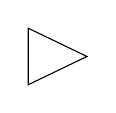
\begin{tikzpicture}[circuit logic US]
              \node (buffer) [buffer gate, draw, logic gate inputs=1, anchor=output] {};
          \end{tikzpicture}
          \\
          \begin{tabular}{|c|c|}
              \hline
              A & Output \\
              \hline
              0 & 0      \\
              1 & 1      \\
              \hline
          \end{tabular}
    \item AND \\
          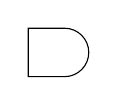
\begin{tikzpicture}[circuit logic US][circuit logic US]
              \node (and) [and gate, draw, logic gate inputs=nn] {};
          \end{tikzpicture}
          \\
          \begin{tabular}{|c|c|c|}
              \hline
              A & B & Output \\
              \hline
              0 & 0 & 0      \\
              0 & 1 & 0      \\
              1 & 0 & 0      \\
              1 & 1 & 1      \\
              \hline
          \end{tabular}
    \item OR \\
          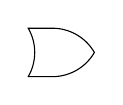
\begin{tikzpicture}[circuit logic US]
              \node (or) [or gate, draw, logic gate inputs=nn] {};
          \end{tikzpicture}
          \\
          \begin{tabular}{|c|c|c|}
              \hline
              A & B & Output \\
              \hline
              0 & 0 & 0      \\
              0 & 1 & 1      \\
              1 & 0 & 1      \\
              1 & 1 & 1      \\
              \hline
          \end{tabular}
    \item NOT \\
          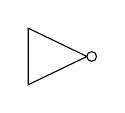
\begin{tikzpicture}[circuit logic US]
              \node (not) [not gate, draw, logic gate inputs=n] {};
          \end{tikzpicture}
          \\
          \begin{tabular}{|c|c|}
              \hline
              A & Output \\
              \hline
              0 & 1      \\
              1 & 0      \\
              \hline
          \end{tabular}
    \item NAND \\
          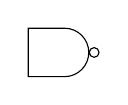
\begin{tikzpicture}[circuit logic US]
              \node (nand) [nand gate, draw, logic gate inputs=nn] {};
          \end{tikzpicture}
          \\
          \begin{tabular}{|c|c|c|}
              \hline
              A & B & Output \\
              \hline
              0 & 0 & 1      \\
              0 & 1 & 1      \\
              1 & 0 & 1      \\
              1 & 1 & 0      \\
              \hline
          \end{tabular}
    \item NOR \\
          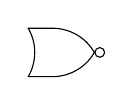
\begin{tikzpicture}[circuit logic US]
              \node (nor) [nor gate, draw, logic gate inputs=nn] {};
          \end{tikzpicture}
          \\
          \begin{tabular}{|c|c|c|}
              \hline
              A & B & Output \\
              \hline
              0 & 0 & 1      \\
              0 & 1 & 0      \\
              1 & 0 & 0      \\
              1 & 1 & 0      \\
              \hline
          \end{tabular}
    \item XOR \\
          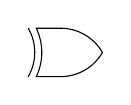
\begin{tikzpicture}[circuit logic US]
              \node (xor) [xor gate, draw, logic gate inputs=nn] {};
          \end{tikzpicture}
          \\
          \begin{tabular}{|c|c|c|}
              \hline
              A & B & Output \\
              \hline
              0 & 0 & 0      \\
              0 & 1 & 1      \\
              1 & 0 & 1      \\
              1 & 1 & 0      \\
              \hline
          \end{tabular}
    \item XNOR \\
          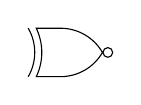
\begin{tikzpicture}[circuit logic US]
              \node (xnor) [xnor gate, draw, logic gate inputs=nn] {};
          \end{tikzpicture}
          \\
          \begin{tabular}{|c|c|c|}
              \hline
              A & B & Output \\
              \hline
              0 & 0 & 1      \\
              0 & 1 & 0      \\
              1 & 0 & 0      \\
              1 & 1 & 1      \\
              \hline
          \end{tabular}
\end{itemize}

\end{document}

%\begin{center}
%    \begin{forest}
%        [0.INTMAX [1.16 [2.12 [3.10] [3.12]] [3.16 [4.14] [4.16]]][4.INTMAX [5.20 [6.18] [6.20]] [6.INTMAX]]]
%    \end{forest}    
%\end{center}